\documentclass[12pt]{article}


\usepackage{apuntes-estilo}
\usepackage{fancyhdr,lastpage}
\usepackage{color,colortbl}
\usepackage{verbatim}

\def\maketitle{

% Titulo 
 \makeatletter
 {\color{bl} \centering \huge \sc \textbf{
 Compilación, Vinculación y Localización\\ 
\large \vspace*{-8pt} \color{black} Programación de Sistemas Embebidos
 \vspace*{8pt} }\par}
 \makeatother


% Autor
 \makeatletter
 {\centering \small 
 	Departamento de Ingeniería de Computadoras \\
 	Facultad de Informática - Universidad Nacional del Comahue \\
 	\vspace{20pt} }
 \makeatother

}

% Custom headers and footers
\fancyhf{} % clear all header and footer fields
\fancypagestyle{plain}{\fancyhf{}}
  	\pagestyle{fancy}
 	\lhead{\footnotesize Compilación, vinculación y localización - Programación de sistemas embebidos}
 	\rhead{\footnotesize \thepage\ }	% ''Page 1 of 2''

\def\ti#1#2{\texttt{#1} & #2 \\ }



\begin{document}

\thispagestyle{empty}
\maketitle
\setlength{\parindent}{0pt}

{\it I consider that the golden rule requires that if I like a program I must share it with other people who like
it. Software sellers want to divide the users and conquer them, making each user agree not to share with
others. I refuse to break solidarity with other users in this way. I cannot in good conscience sign a
nondisclosure agreement or a software license agreement. So that I can continue to use computers
without dishonor, I have decided to put together a sufficient body of free software so that I will be able
to get along without any software that is not free.}
—Richard Stallman, Founder of the GNU Project The GNU Manifesto


En este capítulo se examinan los pasos involucrados en la preparación
del software para la ejecución en un sistema embebido.
También se dan detalles de las herramientas de desarrollo asociadas
al proceso, y se proporciona, como ejemplo, la
construcción del programa Blinking LED estudiado en el Capítulo anterior.

Un detalle importante, útil de aclarar primero, es que la programación
de sistemas embebidos no es muy diferente de la programación
realizada sobre sistemas de propósito general (por ejemplo en PC).
Lo único que realmente cambia en el proceso es que se necesita 
entender la plataforma de hardware destino. Además, cada 
plataforma de hardware es única, por ejemplo, el método de comunicación
de una interfaz serial puede variar de procesador a procesador y de plataforma
a plataforma.
Desafortunadamente, estas diferencias entre las plataformas de hardware
provoca una gran cantidad de complejidad adicional, y es también la razón
por la cual se necesita trabajar mucho más que antes en el proceso de construcción
del software.

Nos enfocaremos en el uso de herramientas de software open source.


\section *{El proceso de compilación}

Cuando las herramientas de compilación se ejecutan en el mismo sistema (host)
que el programa generado (target) las herramientas pueden realizar
varias suposiciones sobre el sistema.
No es el caso en el desarrollo de sistemas embebidos, donde las herramientas
de desarrollo se ejecutan en una máquina (host) diferente a la plataforma
de hardware destino (target).
Cuando la plataforma destino es la misma que la de desarrollo (host), y está
bien definida, las herramientas de
desarrollo de software pueden realizar varias cosas automáticamente.
 
\fcolorbox{black}{grey}{
\parbox[t]{1.0\linewidth}{ \vspace*{0.4cm}
NOTA: la plataforma destino (target) incluye tanto el hardware como así
también el sistema operativo, que conforman el ambiente de ejecución
básico para la aplicación. Si no existe sistema operativo, como es
muchas veces el caso en sistemas embebidos, la plataforma destino
es simplemente el procesador en el cual se ejecuta el  programa.
\vspace*{0.4cm} } }

En cambio, las herramientas de desarrollo para software embebido 
raramente pueden realizar suposiciones sobre la plataforma destino.
En vez de eso, el usuario debe proveer 
conocimiento del sistema a las herramientas, a través 
de mayor cantidad de instrucciones explícitas que lo que haría
si tanto el target como el host fueran la misma plataforma.

El proceso de convertir el código fuente del software embebido
en una imagen binaria ejecutable involucra tres pasos bien distinguidos:

\begin{enumerate}
\item Cada archivo fuente debe ser compilado o ensamblado en un archivo objeto.
\item Todos los archivos objetos del primer paso deben ser vinculados (linked)
juntos para generar un archivo objeto individual, llamado el programa reubicable.
\item Direcciones físicas de la memoria deben ser asignadas a los desplazamientos (offsets)
dentro del programa reubicable en un proceso llamado reubicación (relocation).
\end{enumerate}

El resultado del paso final es un archivo que contiene una imagen binaria
que está lista para ser ejecutada en el sistema embebido.

El proceso recién descripto está representado en la Figura \ref{fig:compilacion}.
Allí se se observan los tres pasos comenzado desde arriba hacia abajo,
en conjunto con las herramientas utilizadas (que aparecen
en los recuadros con esquinas redondeadas).
Estas herramientas de desarrollo toman uno o más archivos como entrada
y producen un archivo individual como salida. 

\begin{figure}
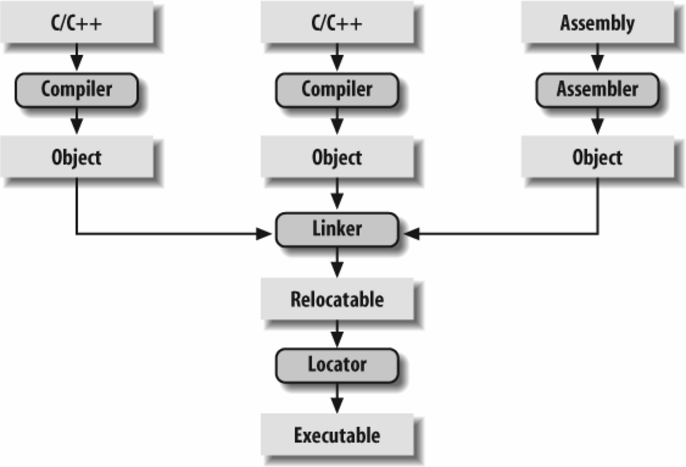
\includegraphics[width=\linewidth]{compilacion.png}
\caption{El proceso de desarrollo de software embebido.}
\label{fig:compilacion}
\end{figure}



Cada paso del proceso de compilación de software embebido
es una transformación realizada por software ejecutado en una computadora
de propósito general. Para distinguir esta computadora de desarrollo (usualmente una 
PC o estación de trabajo UNIX) del sistema embebido destino se utiliza el término host computer.
En esta computadora es donde se ejecuta el compilador, ensamblador, vinculador y se realiza la localización (locator).
Aunque, como ya mencionado, estas herramientas trabajan en conjunto
para producir una imagen binaria que puede ser ejecutada
únicamente en el sistema embebido destino. Esta división de responsabilidades
se representan en la Figura \ref{fig:compilacion2}

\begin{figure}
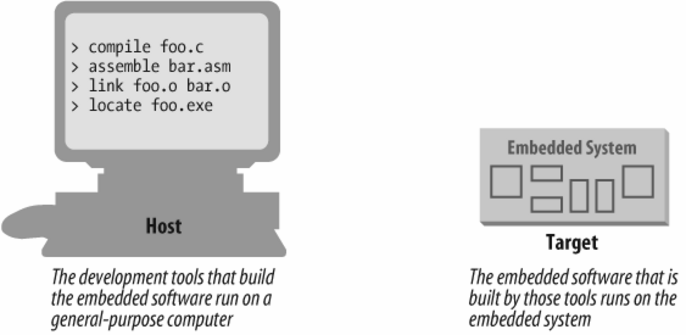
\includegraphics[width=\linewidth]{compilacion2.png}
\caption{Computadora de desarrollo (host) y computador destino (target).}
\label{fig:compilacion2}
\end{figure}

En este libro se utilizan las herramientas de desarrollo del proyecto GNU
(compilador, ensamblador, vinculador y debugger) las cuales son software libre
y tienen extensa documentación en libros, y páginas de manual online en sistemas
Linux y UNIX. Una vez comprendido
el uso de las mismas puede aplicarse los mismos conceptos a herramientas
de desarrollo equivalentes (comerciales o no).

\subsection *{Compilando}

La tarea de un compilador es, principalmente, traducir programas escritos en 
algún lenguaje leíble por personas en un conjunto equivalente
de códigos de operación para algún procesador particular. En ese sentido,
el ensamblador es también un compilador (generalmente se lo llama
compilador de lenguaje ensamblador), pero su tarea es mas sencilla, ya que
realiza una traducción de uno a uno, de nemotécnicos leíble por personas
en sus equivalentes códigos de operación de la CPU. El resto de lo explicado en esta sección
aplica a compiladores y ensambladores. En conjunto, estas herramientas
realizan el primer paso del proceso de construcción de software embebido
ya mencionado.

Por supuesto, cada procesador tiene su propio lenguaje máquina, por lo que
necesita seleccionar un compilador que produzca programas para el procesador
destino específico. En el caso de los sistemas embebidos,  este compilador
casi siempre se ejecuta en la computadora host. Simplemente no tiene sentido,
la mayoría de las veces, ejecutar el compilador en el sistema embebido.
Un compilador que realiza esta tarea -se ejecuta en una plataforma  y produce
código para otra- es llamado un compilador cruzado (cross-compiler). El uso de
un compilador cruzado es una de las características de desarrollo de software
embebido.

El compilador C GNU (gcc) y el ensamblador (as) pueden ser configurados y compilados
como compiladores nativos o compiladores cruzados. Estas herramientas soportan
un impresionante conjunto de combinaciones host-target. El compilador gcc ha sido
portado a todos los sistemas operativos Mac y PC. También, el soporte de procesadores destino
es extenso, e incluye AVR, Intel x86, MIPS, PowerPC, ARM y SPARC. Información
adicional puede ser encontrada online en {\tt http://gcc.gnu.org}.

Cualquiera sea el lenguaje de entrada (C, C++, ensamblador o cualquier otro), la salida
de un compilador cruzado será un archivo objeto. Este es un archivo binario con
formato especial que contiene el conjunto de instrucciones y datos
resultado del proceso de traducción del lenguaje. Aunque partes de este archivo
contiene código ejecutable el archivo objeto no puede ser ejecutado directamente.


El contenido de un archivo objeto puede ser imaginado como una estructura de datos
muy grande y flexible. La estructura del archivo está definida en un formato estándar, 
por ejemplo, Common Object File Format (COFF) o Executable and Linkable Format (ELF).
Si se utiliza más de un compilador (i.e. se está escribiendo diferentes partes de un programa
en diferentes lenguajes fuente) se debe estar seguro que el compilador es capaz
de producir archivos objetos en el mismo formato. En este contexto, gcc soporta 
los dos formatos recién mencionados. Aunque muchos compiladores (y en particular
los que son para ambientes UNIX) soportan formatos de archivo objeto como
COFF y ELF, algunos producen archivos objetos en formatos propietarios.
Si se utilizan compiladores de este último grupo se necesita obtener todas
las restantes herramientas de desarrollo desde el mismo proveedor.


La mayoría de los archivos objetos comienzan con un encabezado que describe las secciones
que siguen. Cada una de esas secciones contienen uno o mas bloques de código o datos que 
provienen de los archivos fuentes. De cualquier manera, el compilador tiene reagrupado
esos bloques en secciones relacionadas. Por ejemplo, gcc agrupa todos los bloques de
código en una sección llamada text, todas las variables globales inicializadas (y sus
valores iniciales) en una sección llamada data, y todas las variables globales sin 
inicializar en una sección llamada bss.

Hay también, usualmente, una tabla de símbolos en el archivo objeto, que contiene
los nombres y las ubicaciones de todas las variables y funciones referenciadas dentro
del archivo fuente. Partes de esta tabla podría estar incompleta, debido a que
no todas las variables y funciones son siempre definidas en el mismo archivo fuente. 
Esos son los símbolos que hacen referencia a variables y funciones definidas en 
otro archivo fuente distinto. Es trabajo del vinculador resolver todas esas referencias
no resueltas.

\subsection *{Vinculando}

Todos los archivos objetos que fueron el resultado del paso uno del proceso deben
ser vinculados. Los archivos objetos individualmente están incompletos, por lo que
alguna de las referencias a variables y funciones internas aún no han sido resueltas.
La tarea del vinculador (linker) es combinar esos archivos objetos, y en el proceso,
resolver todos los símbolos no resueltos.

La salida del vinculador es un nuevo archivo objeto, que contiene todo el código y datos
de los archivos objetos de entrada (en el mismo formato).
Eso es logrado al combinar las secciones text, data y bss de los archivos de entrada.
Cuando el vinculador finaliza, todo el código en lenguaje máquina de todos los archivos
objetos de entrada está en la sección text del nuevo archivo, y todas las variables
inicializadas o no en las secciones nuevas data y bss respectivamente.

Mientras el vinculador está en el proceso de integrar 
los contenidos de las secciones también 
busca los símbolos sin resolver. Por ejemplo, si un archivo objeto contiene 
una referencia no resuelta a  una variable llamada foo, y una variable con 
el mismo nombre está declarada en uno de los archivos objetos, el vinculador
integrará ambas. La referencia no resuelta sera reemplazada con la referencia
a la variable encontrada. Por ejemplo, si foo está ubicada a 14 bytes de desplazamiento
de donde comienza la sección de datos, su entrada en la tabla de símbolos ahora
contendrá esa dirección.

El vinculador (ld) GNU está portado a todas las mismas plataformas en donde
fue portado el compilador GNU (gcc). Esta es una herramienta de la linea de comandos
que toma como argumentos de entrada todos los nombres de los archivos objeto, 
y posiblemente bibliotecas a ser vinculadas.
Con software embebido, un archivo objeto especial que contiene el código de 
inicialización (startup code), debe también ser incluido dentro de esta
lista de archivos que procesa ld (se darán mas detalles sobre el código
de inicialización en secciones siguientes). Finalmente, cabe mencionar
que el vinculador GNU tiene un lenguaje de scripting que puede ser utilizado
para controlar cómo debe ser el archivo objeto de salida.

Si el mismo símbolo es declarado en más de un archivo objeto de los que 
procesa ld entonces se finalizará el proceso inmediatamente, mostrando un mensaje
de error al usuario explicando el error de programación.

Por el contrario, si una referencia a un símbolo queda sin resolver luego de
procesado todos los archivos objetos el vinculador intentará resolver la misma
por su cuenta.
La referencia podría ser una función, tal como memcpy, strlen o malloc, que son
parte de la biblioteca de C estándar, por lo que ld abrirá cada uno de las
bibliotecas descriptas como argumentos en la línea de comandos (en el orden
en que se mencionaron) y examina sus tablas de símbolos. 
Si el vinculador descubre una función o variable con ese nombre la referencia
será resuelta agregando el código y datos asociados a esta referencia en el 
archivos objeto de salida.

\fcolorbox{black}{grey}{
\parbox[t]{1.0\linewidth}{ \vspace*{0.4cm}
NOTA: Este último procedimiento realizado por ld es únicamente para vinculación
estática. Cuando se realiza vinculación dinámica de bibliotecas el código 
y datos asociados con la rutina de biblioteca no son insertadas dentro
del programa.
\vspace*{0.4cm} } }

\fcolorbox{black}{grey}{
\parbox[t]{1.0\linewidth}{ \vspace*{0.4cm}
NOTA2: El vinculador GNU utiliza vinculación selectiva, lo cual mantiene
otras funciones sin referenciar afuera de la imagen de salida
del vinculador.
\vspace*{0.4cm} } }

Desafortunadamente, las rutinas de la biblioteca estándar frecuentemente requiere 
algunos (o muchos) cambios antes que pueda ser utilizada en un sistema embebido.
Un problema es que las bibliotecas estándar provistas con la mayoría de las 
suites de herramientas de desarrollo de software vienen únicamente en forma objeto.
Raramente tienes acceso al código fuente de la biblioteca para hacer los 
cambios necesarios. Pero, existen algunas alternativas. Una de ellas es
la provista por la compañía Cygnus (la cual es ahora parte de Red Hat),
la cual creó una versión freeware de la biblioteca de C estándar para utilizar 
en sistemas embebidos.
Este paquete es llamado newlib. Simplemente se necesita descargar el código fuente
para esta biblioteca desde la web (actualmente ubicada en {\tt http://sourceware.org/newlib}),
implementar unas pocas funciones especificas para el hardware destino y compilar.
La biblioteca puede luego ser vinculada con nuestras aplicaciones embebidas
para resolver cualquier llamada a la biblioteca estándar sin resolver previamente.

Luego de integrar todas las secciones de código y datos, y de resolver todas
las referencias a símbolos, el vinculador genera un archivo objeto que es
una copia 'reubicable' (relocatable) especial del programa. En otras palabras,
el programa ya está completo, con la excepción de una cosa: todavía
resta definir las direcciones de memoria asignadas a las secciones de código y 
datos. Si no se estuviera realizando el proceso para ejecutarse en un 
sistema embebido entonces el programa estaría listo para ejecutarse.

Pero, los programadores de sistemas embebidos aún deben realizar una
tarea más en este punto, ya que 
las direcciones de los símbolos en el proceso de vinculación son relativas.
Aun si tu sistema embebido incluye un sistema operativo es necesario
que la imagen binaria final sea ubicada de manera absoluta (y no relativa).
De hecho, si existe un sistema operativo en el proyecto del sistema embebido,
el código y datos del mismo mayormente estará en el programa reubicable 
también.
La aplicación embebida completa -incluyendo el sistema operativo- es
frecuentemente vinculada en conjunto y ejecutada como una imagen binaria
individual.

\subsubsection *{Código de inicialización (Startup code)}

Una de las acciones que las herramientas de software tradicional realizan
es agregar automáticamente el código de inicialización: un pequeño bloque
de código en lenguaje ensamblador que prepara el camino para la ejecución
del software escrito en un lenguaje de alto nivel. Cada lenguaje de alto
nivel tiene un conocimiento propio acerca del ambiente de ejecución.
Por ejemplo, programas escritos en C utilizan una pila (stack). Espacio
para la pila tiene que ser reservado y ubicado antes de que el software escrito
en C pueda ser ejecutado apropiadamente. Esa es una de las responsabilidades
asignadas al código de inicialización para programas en C.

La mayoría de los compiladores cruzados (cross-compilers) para sistemas
embebidos incluyen un archivo en lenguaje ensamblador llamado startup.asm, crt0s
(abreviatura de C runtime), o algún nombre similar. La ubicación y contenido de este
archivo está usualmente descripto en el manual suministrado con el compilador.

El código de inicialización para programas en C usualmente consiste de la siguiente
lista de acciones:

\begin{enumerate}
\item Deshabilitar las interrupciones.
\item Copiar cualquier dato inicializado desde la ROM a RAM.
\item Poner en cero el área de datos sin inicializar.
\item Reservar espacio e inicializar la pila.
\item Inicializar el puntero de pila del procesador.
\item Llamar a main.
\end{enumerate}

Típicamente, el código de inicialización también incluye unas pocas
instrucciones después de llamar a main. Estas instrucciones serán ejecutadas
sólo en el caso de que el programa en el lenguaje de alto nivel finalice (i.e.
la llamada a main retorne). Dependiendo de la naturaleza del sistema embebido
se podría utilizar estas instrucciones para realizar un halt del procesador, 
reiniciar el sistema entero, o transferir el control a una herramienta
de verificación (debug tool).

En general, el código de inicialización no es insertado automáticamente al desarrollar sistemas embebidos. El
programador debe ensamblar el código fuente del mismo e incluir el archivo objeto resultante a la 
lista de archivos de entrada del vinculador explícitamente. Además, el programador
podría necesitar indicarle al vinculador una opción en la línea de comandos especial
para prevenir que ld intente insertar el código de inicialización provisto
por el toolchain.
Código de inicialización funcional para una variedad de procesadores puede
ser encontrado en el paquete GNU llamado libgloss.


\fcolorbox{black}{grey}{
\parbox[t]{1.0\linewidth}{ \vspace*{0.4cm}

{\sf Debug Monitors}

En algunos casos, un debug monitor (o ROM monitor) es el primer código
ejecutado cuando la placa es encendida. En el caso del arduino pro mini
existe un bootloader provisto por el proyecto Arduino que se ejecuta en primer lugar.
Esta pieza de software puede ser utilizada
para descargar software, y ubicar el mismo en la memoria FLASH de la placa, en la dirección 0x00.
Si el bootloader no recibe ordenes desde el puerto serial simplemente ejecuta la aplicación
actual en FLASH.
\vspace*{0.4cm} } }

\subsection *{Localización}

La herramienta que realiza la conversión de un programa reubicable a
una imagen binaria ejecutable es llamada reubicador (locator).
Este realiza el paso mas fácil del proceso de compilación. De hecho, 
el programador debe hacer la mayoría del trabajo en este paso, informando
detalles acerca de la memoria de la plataforma destino, como entrada.
El reubicador utiliza esta información para asignar direcciones
de memoria físicas a las secciones de código y datos dentro del programa
reubicable. Finalmente, el reubicador produce un archivo de salida que contiene
una imagen de memoria binaria que puede ser descargada dentro del sistema
embebido destino.

Cuando se escribe software para una computadora de propósito general o
sistema embebido, en algún punto las secciones del programa reubicable
deben tener asignadas direcciones concretas. Algunas veces el software
que está en la computadora destino realiza esta tarea (por ejemplo un sistema
operativo o bootloader). No es el caso del arduino pro mini, aunque por suerte,
las herramientas de desarrollo GNU para arquitectura AVR traen estos detalles 
incorporadas, como así también el código de inicialización para la mayoría
de los microcontroladores de AVR de Atmel.
Cuando se realiza el paso de vinculación y localización para arquitectura AVR,
con el vinculador GNU ld, se agrega el código de inicialización y se 
resuelven las direcciones reales de acuerdo al microcontrolador destino.

Si se debe suministrar, manualmente, información de la memoria de la plataforma destino
al vinculador  GNU, se debe escribir un linker script.
Estos scripts son utilizados algunas veces para controlar el orden exacto de
las secciones de código y datos dentro del programa reubicable, y establecer
la ubicación física de cada sección en memoria.


Debajo se muestra un ejemplo extraído y resumido de un linker script
para un microcontrolador Atmel de arquitectura AVR. El archivo script
completo es utilizado por avr-ld en la compilación el ejemplo Blinking LED
presentado en el Capítulo 3.

\begin{verbatim}
MEMORY
{
  text   (rx)   : ORIGIN = 0, LENGTH = 8K
  data   (rw!x) : ORIGIN = 0x800100, LENGTH = 0
}
SECTIONS
{
  .text 0 :
  {
    *(.vectors)
    KEEP(*(.vectors))
     __ctors_start = . ;
     *(.ctors)
    *(.text)
  }
  .data        0 :
  {
    *(.data)
    *(.rodata)  /* We need to include .rodata here if gcc is used */
  }
  .bss  0 :
  {
    *(.bss)
    *(COMMON)
  }

...

}
\end{verbatim}

El script informa al reubicador incluido en el vinculador GNU acerca de las ubicaciones
físicas de las secciones del programa en la memoria del sistema embebido destino.
El script instruye a ld a ubicar la sección de texto en la dirección física 0x00,
y a la sección de datos en la dirección 0x800100.

Nombres en el archivo de comandos del vinculador que comienzan con un guión bajo
(ejemplo \_\_ctors\_start) pueden ser referenciado similarmente a variables ordinarias
desde dentro de el código fuente. El vinculador utilizará estos símbolos
para resolver referencias en los archivos objeto de entrada.
Por lo que, por ejemplo, podría existir una parte del software embebido (usualmente
dentro del código de inicialización) que copia valores iniciales de las variables
inicializadas desde ROM a la sección data en RAM.

Un script para el vinculador puede también utilizar varios otros comandos
para instruir al vinculador a que realice otras operaciones.
Información adicional y opciones de los archivos script para el vinculador GNU ld
puede ser leída desde http://www.gnu.org.

La salida de este paso final del proceso de compilación es una imagen binaria
conteniendo direcciones físicas para el sistema embebido destino específico.
Esta imagen binaria ejecutable puede ser descargada a la memoria del sistema embebido.

Afortunadamente, como se mencionó anteriormente, las herramientas de desarrollo
GNU para microcontroladores AVR pueden realizar este ultimo paso automáticamente
(para casi todos lo microcontroladores existentes de esta arquitectura).

\section *{Compilando el programa Blinking LED}

En esta sección se muestra un ejemplo del procedimiento de compilación 
para el microcontrolador Atmel AVR atmega328p (placa arduino pro mini).
Si se utiliza otra plataforma, un proceso similar debería ser ejecutado
utilizando las herramientas y convenciones que acompañan al hardware.

\subsection {Compilar, ensamblar y vincular}

El ejemplo Blinking LED consiste de dos archivos fuentes : led.c y blink.c.
El primer paso en el proceso es compilar estos dos archivos.
La estructura básica para el compilador gcc es :

\begin{verbatim}
avr-gcc [opciones] archivo
\end{verbatim}

Compilamos y vinculamos nuestro programa con :

\begin{verbatim}
avr-gcc -Os -DF_CPU=16000000UL -mmcu=atmega328p -c -o led.o led.c
avr-gcc -Os -DF_CPU=16000000UL -mmcu=atmega328p -c -o blink.o blink.c
avr-gcc -mmcu=atmega328p led.o blink.o -o led.elf
\end{verbatim}

Las opciones utilizadas son :

\begin{itemize}
\item -D para definir una macro. En este caso, es una macro muy utilizada
con el compilador avr-gcc, ya que define la velocidad del reloj del microcontrolador
a utilizar.
\item -mmcu= para seleccionar el modelo del microcontrolador destino 
\item -c compilar y ensamblar, pero no vincular
\end{itemize}


\fcolorbox{black}{grey}{
\parbox[t]{1.0\linewidth}{ \vspace*{0.4cm}
NOTA: En el ejemplo se invoca  a gcc durante el proceso de vinculación.
Esto es debido a que el compilador gcc puede invocar al vinculador indirectamente.
Cuando se compila de esta manera, gcc se asegura que las versiones correctas
de ciertas bibliotecas (llamadas multilibs) sean vinculadas con llamadas
introducidas por las configuraciones del toolchain. En algunos casos, si el vinculador ld es invocado directamente y no gcc, el conjunto correcto de multilibs deben
ser especificados en la linea de comandos, para asegurar que la imagen sea
vinculada apropiadamente.
\vspace*{0.4cm} } }

El orden de los archivos objetos determinan su ubicación en memoria.
Debido a que no estamos vinculando ningún código de inicialización explícitamente
el orden de los archivos objetos es irrelevante.
Si se incluyera código de inicialización se debe ubicar el archivo objeto 
en la dirección apropiada. El archivo script para el vinculador puede ser 
utilizado para especificar donde debe residir la rutina de inicialización
en memoria. Además, puede utilizar el archivo script para 
especificar las direcciones exactas para otros código o datos, pero debe
verificar si es realmente necesario o no.

Como se observa en el comando de vinculación, los dos archivos objetos -led.o y blink.o-
son los últimos argumentos de la linea de comandos para el vinculador.
El resultado de este comando es la creación de la imagen binaria ejecutable
en formato ELF, llamada led.elf.

\subsection *{Dar formato al archivo de salida}

En ciertos casos, el archivo binario ejecutable ELF producido en el 
ejemplo de la sección anterior es suficiente para descargar en el sistema 
embebido y ejecutar. En otros casos (como lo es para el arduino pro mini
y su bootloader) se necesita dar formato, para la plataforma destino,
 a la imagen obtenida
en el proceso de compilación.

Para nuestra plataforma de ejemplo necesita utilizar la herramienta
objcopy, que es un programa de binutils.
objcopy es capaz de copiar el contenido de un archivo objeto en otro 
archivo objeto, pero con diferente formato.
Lo utilizaremos en nuestro ejemplo de esta manera :

\begin{verbatim}
 # avr-objcopy -O ihex -R .eeprom led.elf led.hex
\end{verbatim}

En este caso, lo utilizamos para convertir el programa Blinking LED 
en formato ELF a una imagen en formato Intel Hex. Intel Hex 
es un formato de archivo ASCII muy utilizado en algunas plataformas
para descargar y almacenar imágenes binarias.

El comando utiliza la opción -O ihex para especificar el formato 
de archivo de salida como Intel Hex. El archivo de entrada es led.elf
y objcopy se encarga de determinar el tipo de archivo. El archivo de salida
será un nuevo archivo llamado led.hex

Algunas otras herramientas de binutils GNU son útiles para obtener 
información acerca de la imagen binaria construida.
Por ejemplo, el utilitario size, el cual lista el tamaño de las secciones
para un archivo objeto. El siguiente ejemplo es presentado
para nuestro programa Blinking LED construido :

\begin{verbatim}
# avr-size led.elf
   text	   data	    bss	    dec	    hex	filename
    200	      0	      0	    200	     ca	led.elf
\end{verbatim}

El programa Blinking LED contiene 200 bytes utilizados para la sección de text, y
ningún byte para las secciones data y bss. La columna dec muestra el tamaño
total de la imagen, en decimal, y la columna hex en hexadecimal.





\section*{Referencias}

Michael Barr. Programming Embedded Systems in C and C++ 1st Edition. ISBN-13: 978-1565923546
ISBN-10: 1565923545. O'Reilly Media; 1 edition (February 9, 1999)




\subsection*{Licencia y notas de la traducción}

Este apunte es una traducción del libro de referencia, para
ser utilizado como apunte en la materia de grado
'Programación de Sistemas Embebidos' de la Facultad de Informática,
Universidad Nacional del Comahue.
Se han realizado modificaciones
al contenido para aclarar ciertos detalles o agregar partes nuevas.
 También se han
modificado todos los archivos fuentes de código, ya que fueron
portados a la plataforma Atmel atmega328.

Autores : \\
Rafael Ignacio Zurita ({\tt rafa@fi.uncoma.edu.ar}) \\
Rodolfo del Castillo ({\tt rdc@fi.uncoma.edu.ar})

\fcolorbox{black}{grey}{
\parbox[t]{1.0\linewidth}{ \vspace*{0.4cm}
Esta es una obra derivada del libro de referencia que aún NO ha obtenido permiso de publicación.
\vspace*{0.4cm} } }




\include{licGASL}

\end{document}
